%!TEX root = ../main.tex

\par
In order to generate more data from the limited real-world data available, I can add Gaussian noise to existing data.
One way to do so is simply adding Gaussian noise to each point in a track.
A more complex way is generating random walks of the same length, and then add them pointwise to the track.
I will analyze how realistic the data generated by these methods are, and use the larger dataset to examine the quality of my estimators.

\par
The first way to add noise to a track is to just independently add Gaussian noise to each point.
Let $A=[(\vec{x}_{1}),\ldots,(\vec{x}_{n})]$ (with $\vec{x}_{i}\in\R^{2}$) be the track of a hurricane.
For $i=1,\ldots,n$, let $\varepsilon_{i}\sim\mathcal{N}(\mu,\Sigma)$, where $\mu\in\R^{2}$ and $\Sigma\in\R^{2\times{}2}$ are some mean and covariance.
Then our new hurricane track is
\[
	A'=[\vec{x}_{1}+\varepsilon_{1},\ldots,\vec{x}_{n}+\varepsilon_{n}]
\]

\par
A more advanaced way to add noise to a track is to compute a Gaussian random walk of the same length as the track, and then add them together.
Let $A$ be the track of the hurricane as before.
For $i=1,\ldots,n$, let $\varepsilon_{i}\sim\mathcal{N}(\vec{x}_{i-1}+\varepsilon_{i-1},\Sigma)$ and $\varepsilon_{0}\sim\mathcal{N}(\mu,\Sigma)$ for some initial mean $\mu$ and covariance $\Sigma$.
Once again, our new hurricane track is
\[
	A'=[\vec{x}_{1}+\varepsilon_{1},\ldots,\vec{x}_{n}+\varepsilon_{n}]
\]

\par
Investigating the means and covariances that would be mimic real-world data is beyond the scope of this paper, but would represent an interesting direction of future work.
For now, I keep $\mu=0$, and let $\Sigma=0.1I$, for the purposes of comparing the two methods of adding noise.
Given every hurricane from 1970 through 2018, I make duplicate copies and add noise from both methods.
In Table~\ref{tab:noise_landfalls}, we measure the number of direct landfalls from each category, and compare the two noised totals to the original.
(A direct landfall is where the epicenter of the storm directly passes over land -- this allows us to use basemap software to directly determine whether or not a hurricane track with added noise has made landfall.) We find that both methods of adding noise to hurricane data preserve the average number of direct landfalls to a high degree of accuracy.

\begin{table}[t]
	\centering
	\begin{tabular}{|c|c|c|c|} \hline
		& \begin{tabular}{c}
			Number of\\
			Landfalls $l$
		\end{tabular} & \begin{tabular}{c}
			Number of\\
			Hurricanes $n$
		\end{tabular} & $l/n$\\ \hline
		Original Data & 81 & 798 & 0.102\\ \hline
		Gaussian Noise & 80 & 798 & 0.100\\ \hline
		Random Walk & 85 & 798 & 0.107\\ \hline
	\end{tabular}
	\caption{Comparing the number of direct landfalls}
	\label{tab:noise_landfalls}
\end{table}

\begin{figure}
	\centering
	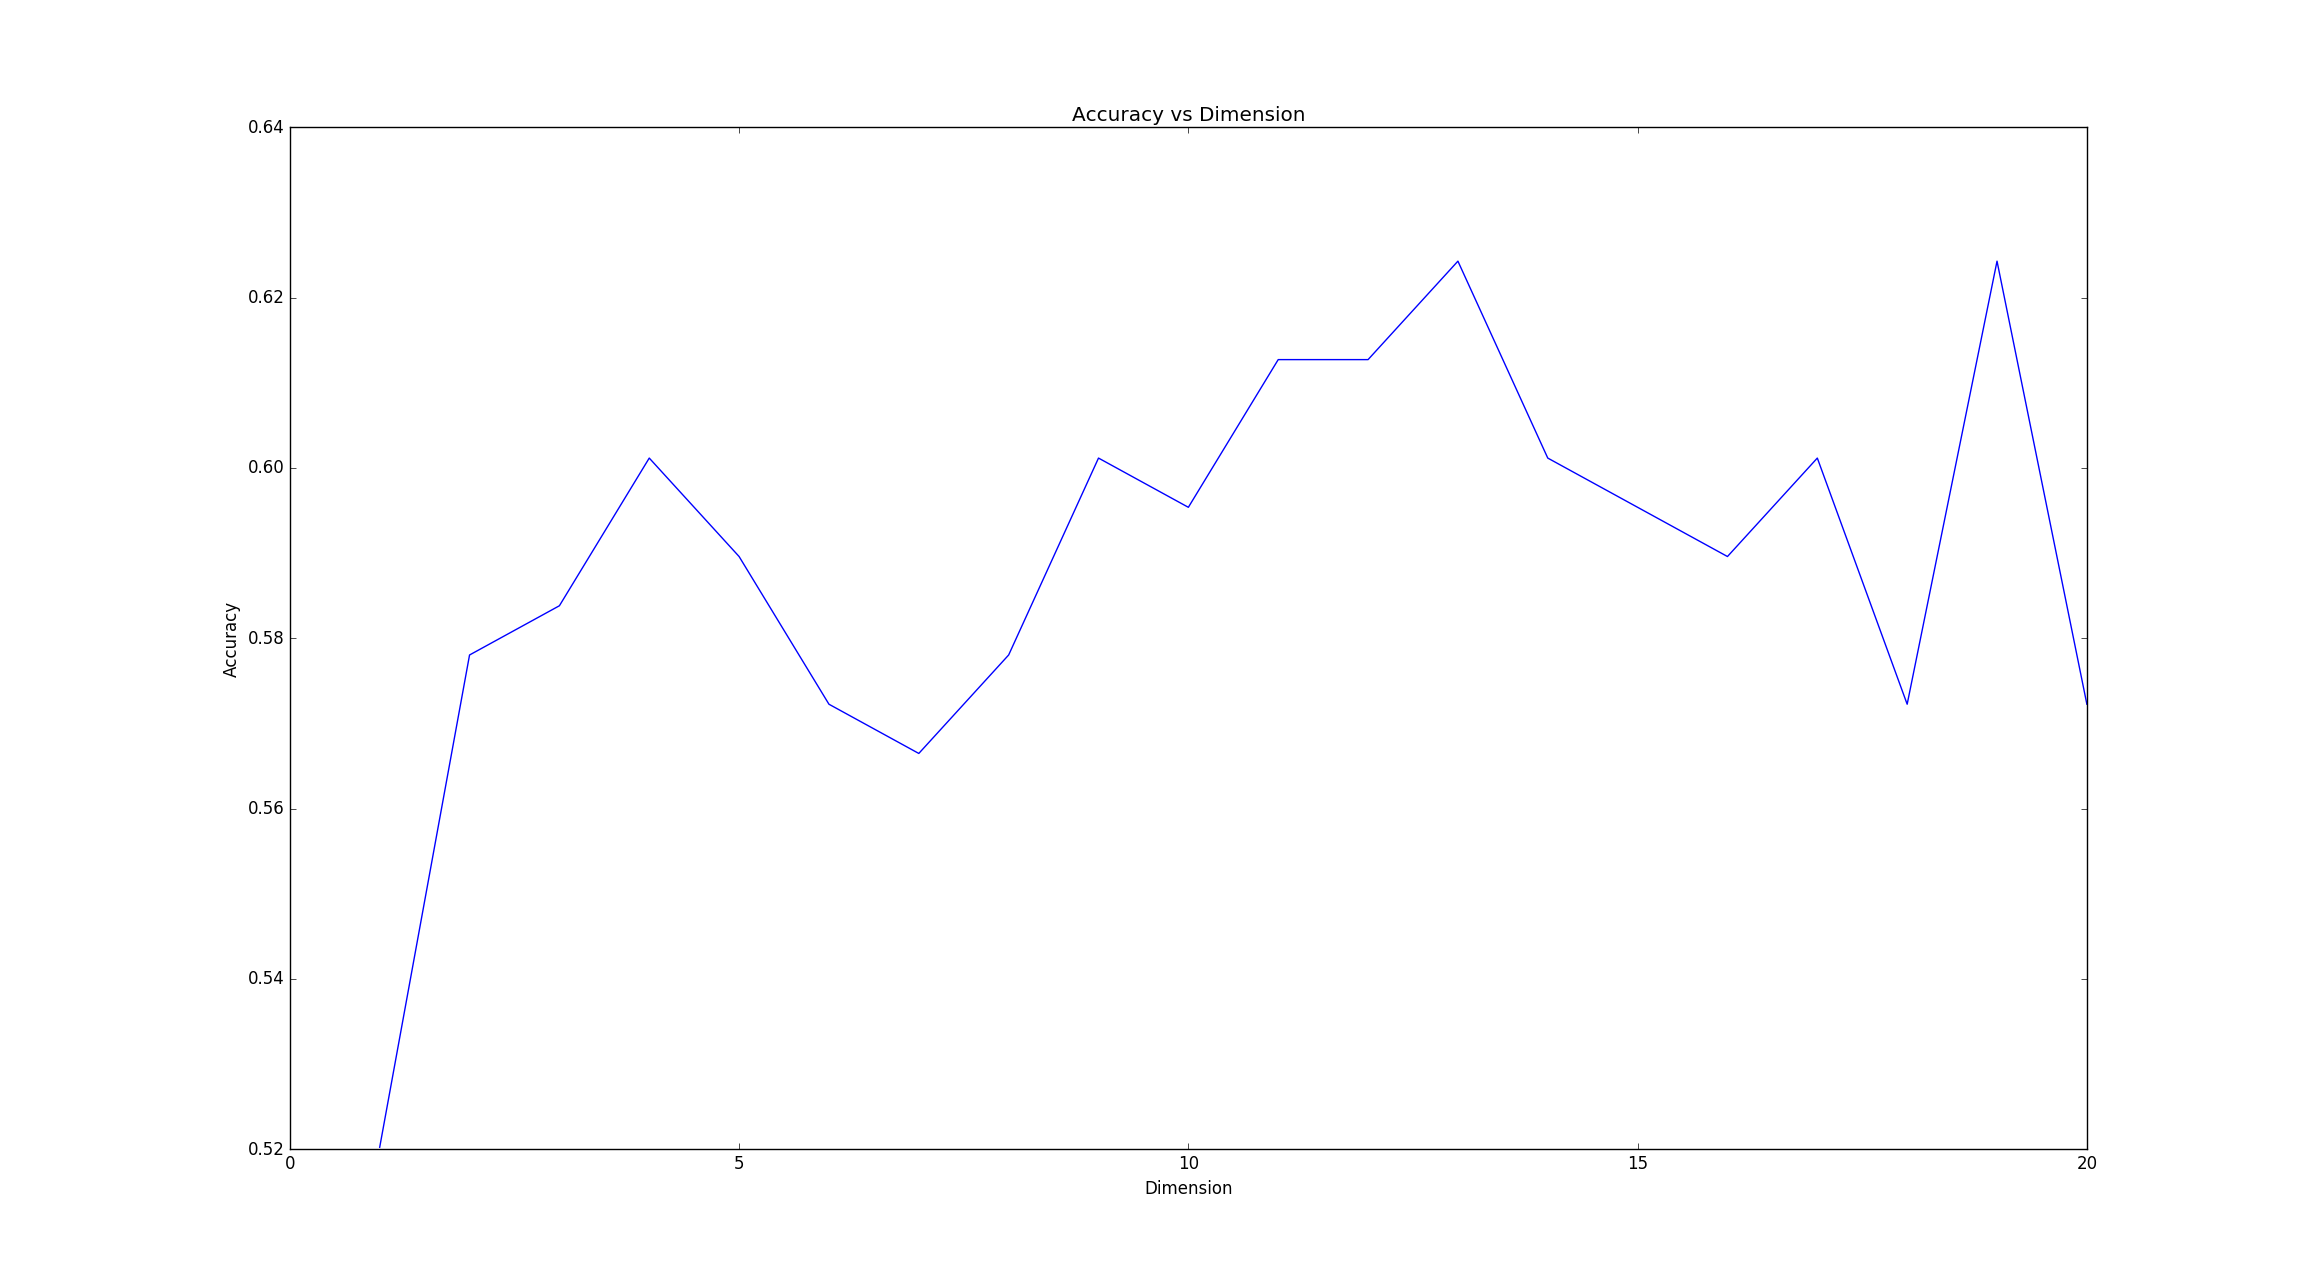
\includegraphics[width=\linewidth]{images/accuracy_vs_dimension.png}
	\caption{A plot of accuracy of the estimator versus the number of dimensions the hurricanes are embedded into by KPCA.}
	\label{fig:dimensions}
\end{figure}

\begin{figure}
	\centering
	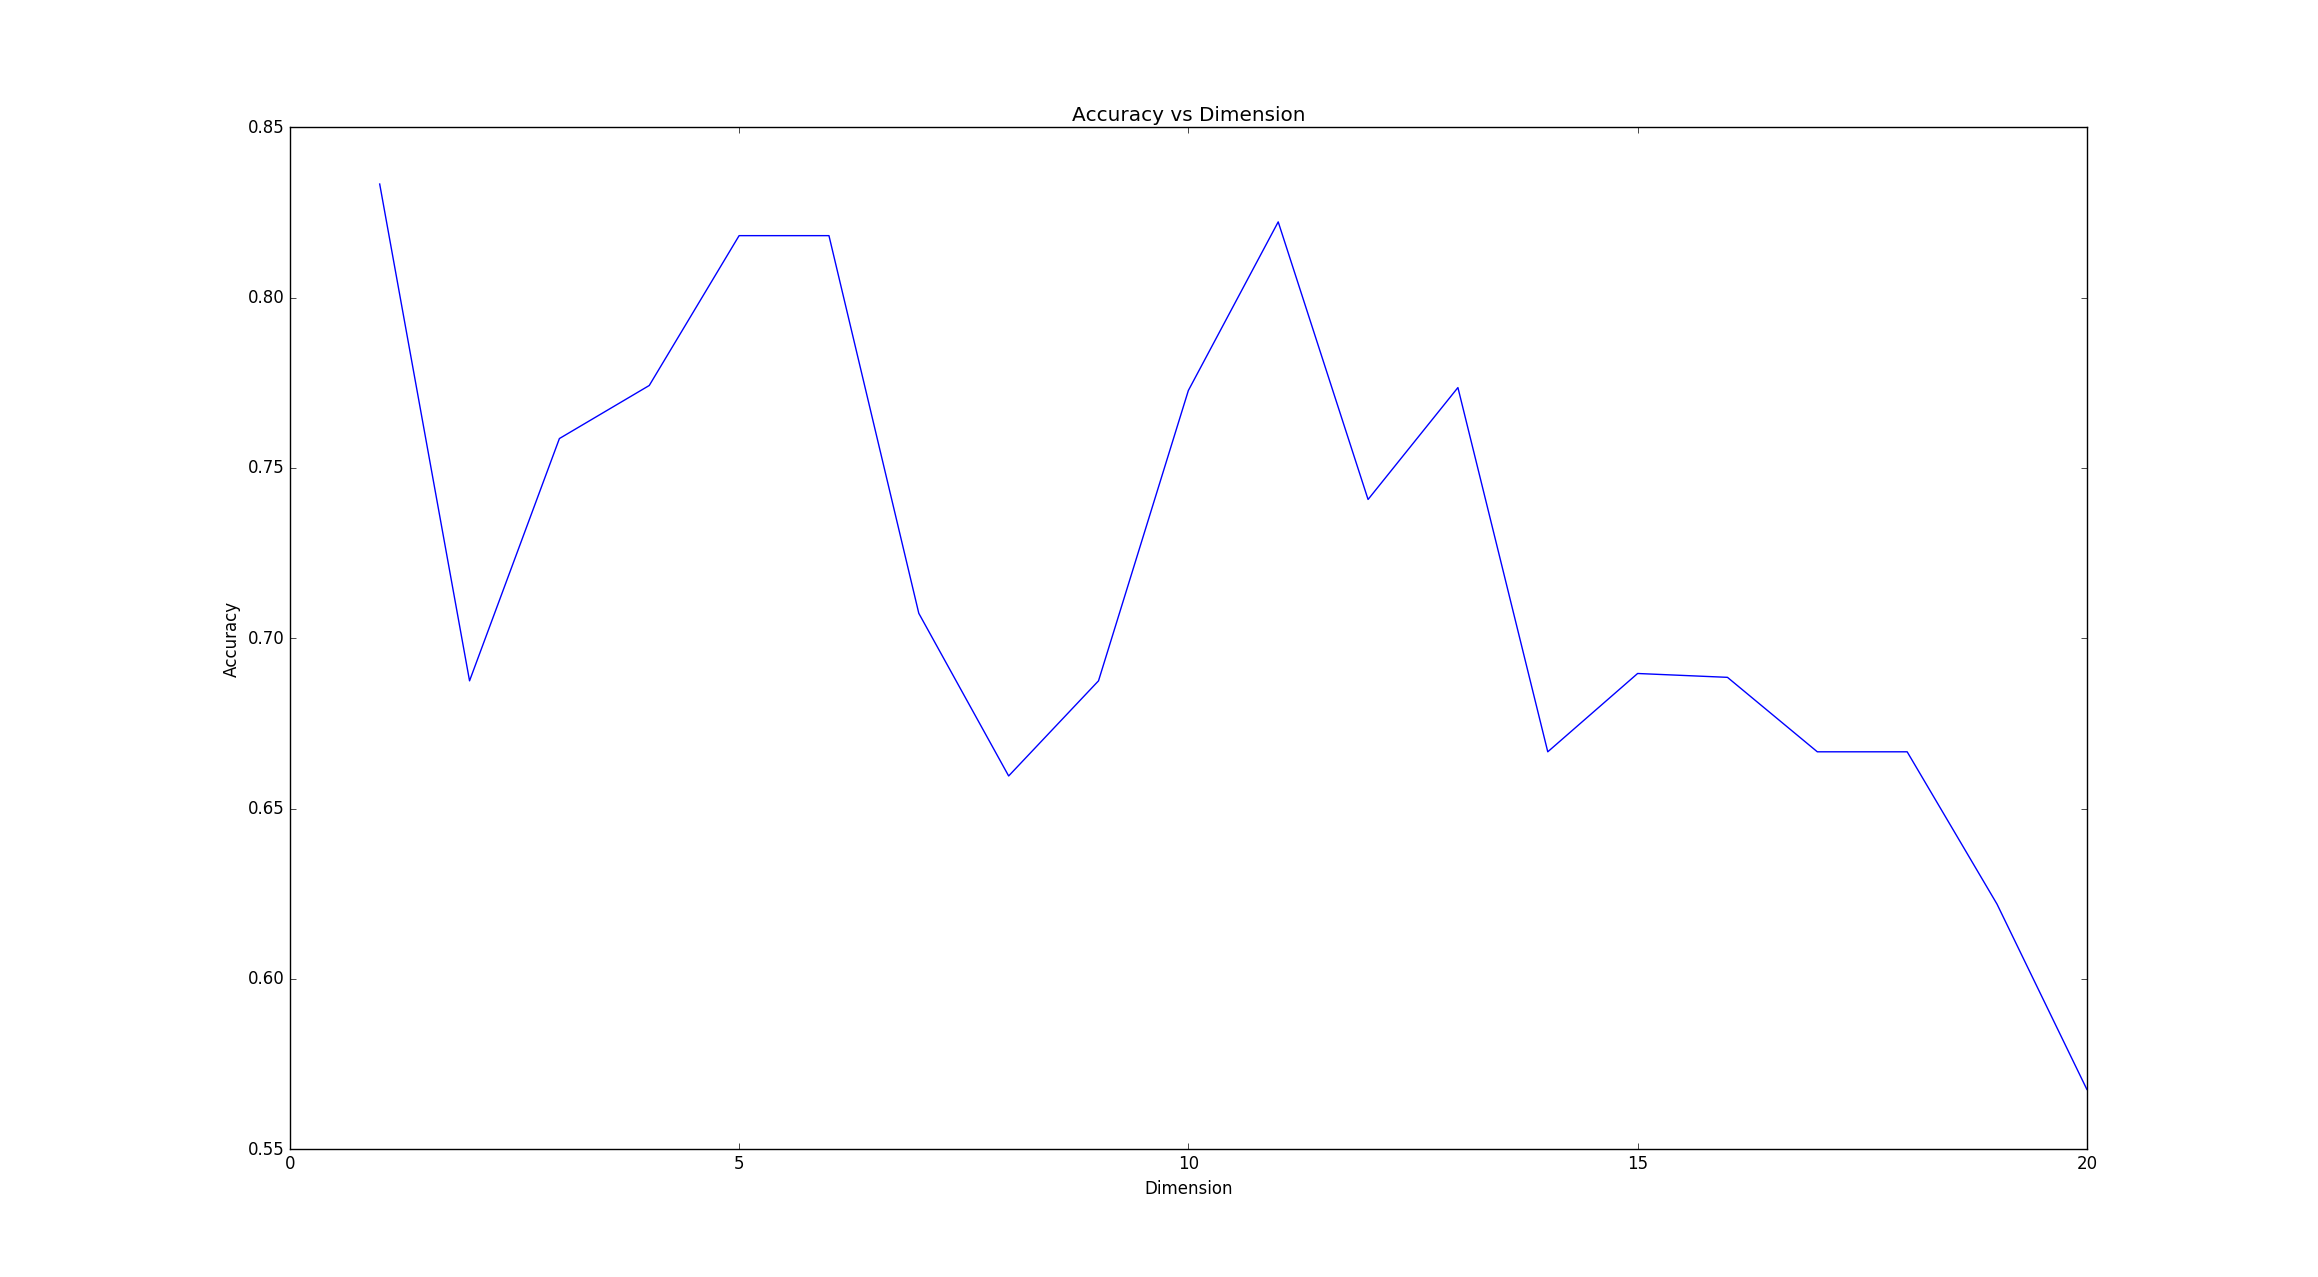
\includegraphics[width=\linewidth]{images/reliable_accuracy_vs_dimension.png}
	\caption{A plot of accuracy of the estimator for only points in which it has high confidence (at least $90\%$) versus the number of dimensions the hurricanes are embedded into by KPCA.}
	\label{fig:confident_dimensions}
\end{figure}

\par
Although quantitatively, both simulation methods have similar results, Figure~\ref{fig:different_noise} provides the basis of a qualitative comparison of the two ways of adding noise.
Specifically, it's clear that adding noise via random walk better accomplishes the goal of producing realistic hurricanes.
The simulated tracks from the random walk method are smoother than those of the pointwise noise method, and they tend to diverge further from the seed hurricane track.